\section{万有引力}

\subsection{引力势能}

\begin{proset}
    某兴趣小组设想了一种探测器发射、卫星回收一体化方案：\ding{172}将卫星携带一探测器发射到半径为\(r_0\)的圆轨道上绕地球做匀速圆周运动。\ding{173}在轨道上某点启动辅助动力装置短暂工作（工作时消耗的气体质量忽略不计），将探测器沿运动方向射出后，探测器恰可脱离地球，而卫星沿原方向绕地球做椭圆运动且恰好未撞到地面。\ding{174}想办法回收卫星。

    \noindent 已知质量分别为\(M_1\)、\(M_2\)的两个质点相距为\(r\)时的引力势能为\(E_p = - G \frac{M_1M_2}{r^2}\)，其中\(G\)为引力常量。已知地球质量\(M\)和地球半径\(R\)，不计空气阻力及其他天体的作用。
    \begin{enumerate}[(1)]
        \item 求卫星和探测器绕圆形轨道运动的周期\(T_0\)、线速度大小\(v_0\)；
        \item 求发射探测器后，卫星第一次运动到地球最近位置经历的时间\(t\)；
        \item 为完成上述任务，某同学认为：\ding{172}应确定卫星与探测器的质量之比\(k\)；\ding{173}还应确定辅助动力装置短暂工作过程中气体燃料提供的能量\(E\)。仅根据题设条件，请你用方程来分析判断确定\(E\)和\(k\)。
    \end{enumerate}
\end{proset}
\begin{answer}
    （1）\(v_0 = \sqrt{\frac{GM}{r_0}}\)\quad \(T_0 = 2\pi \sqrt{\frac{r_0^3}{GM}}\)（2）\(t = \frac{\pi}{2} \sqrt{\frac{(R + r_0)^3}{2GM}}\)（3）可求\(k\)，不可求\(E\)

    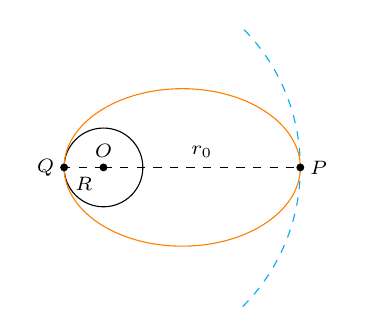
\begin{tikzpicture}[font=\scriptsize]
        \draw (0,0) circle(.5);
        \draw[dashed,cyan] (-45:2.5) arc(-45:45:2.5);
        \draw[orange] (1,0) ellipse(1.5 and 1);
        \draw[dashed] (0,0)node[above]{\(O\)}--node[above]{\(r_0\)}(2.5,0)node[right]{\(P\)} (0,0)--node[below]{\(R\)}(-.5,0)node[left]{\(Q\)};
        \foreach \c in {(0,0),(2.5,0),(-.5,0)}
            \fill \c circle(.05);
    \end{tikzpicture}

    （3）卫星质量为\(m_1\)在椭圆轨道上运动时机械能守恒：\(r_0 v_P = R v_Q\)
    \[
        \frac{1}{2}m_1 v_P^2 +( -  \frac{GMm_1}{r_0^2}) = \frac{1}{2}m_1 v_Q^2 +( - \frac{GMm_1}{R^2})
    \]

    探测器质量为\(m_2\)恰可脱离地球：\(\frac{1}{2}m_2 v_2^2 + (- \frac{GMm_2}{r_0^2}) = 0\)

    卫星与探测器在分离过程中动量守恒：\((m_1 + m_2)v_0 = m_1 v_P + m_2v_2\)

    由上述方程联立可求出\(k\)

    分离过程中能量守恒：\(\frac{1}{2}(m_1 + m_2)v_0^2 + E = \frac{1}{2}m_1 v_P^2 + \frac{1}{2}m_2 v_2^2\)

    缺失\(m_1\)或\(m_2\) 的值，故不可求\(E\)
\end{answer}